\section{V-BLAST}
\subsection{V-BLAST概述}
V-BLAST(Vertical Bell Labs Layered Space-Time)是贝尔实验室提出的一种利用垂直结构来达到极高数据传输速率的无线通信技术。这种技术在一个带限无线信道内,通过多天线技术充分利用空间复用,使得信道容量随着天线数的增加呈线性增长,有着极高的频谱效率。一个典型的V-BLAST MIMO系统的结构图如下:
\begin{figure}[H]
	\centering
	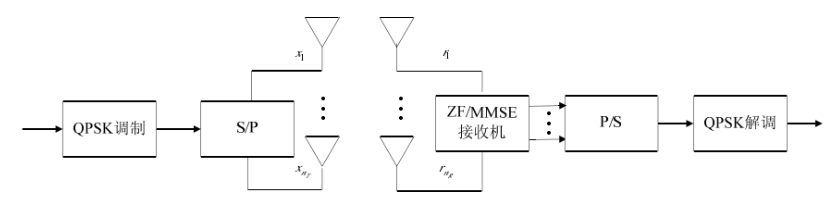
\includegraphics[scale=0.7]{vblast}
	\caption{V-BLAST系统结构图。}
	\label{MIMO}
\end{figure}

\subsection{V-BLAST检测算法}
V-BLAST在接收端对信号进行恢复所使用的检测算法主要有\textbf{迫零(Zero Force)算法}(以下简称\textbf{ZF算法}),\textbf{最小均方误差(Minimal Mean Square Error)算法}(以下简称\textbf{MMSE算法})和\textbf{ML算法}三种。其中ML算法较为复杂,这里不作讨论。

\subsubsection{ZF算法}
假设在接收端信道状态信息(CSI)是已知的,即信道转移矩阵$H$是已知的。ZF检测算法主要是基于Guass-Markov定理,其数学描述为一个最小二乘问题:
\[
\min\Vert r-H\hat{x}\Vert_2^2\quad
\]
其中$\hat{x}$是估计得到的发送信号。\par
令$\frac{\partial}{\partial x}(r-H\hat{x})^T(r-H\hat{x})=0$,即可得到最小二乘问题的闭式解:
\[
\hat{x}_{ZF}=H^\dagger r
\]
其中$H^\dagger=(H^TH)^{-1}H^T$为$H$的伪逆(Moore–Penrose pseudo inverse)。\par
根据Guass-Markov定理:在给定经典线性回归的假定下,最小二乘估计量LSE是具有最小方差的线性无偏估计量(MVUE)。当经典假定成立(即$r$与$x$满足线性变换关系$H$)时,我们不需要再去寻找其它无偏估计量,没有一个会优于LSE估计量。也就是说,如果存在一个好的线性无偏估计量,这个估计量的方差最多与LSE的方差一样小,不会小于LSE的方差。\par
ZF检测的设计目标是在不考虑噪声的情形下,完全消除天线间干扰,因此不需要噪声的统计特性。并且计算方法较为简单,直接通过求解信道矩阵的伪逆即可得到(复杂度$O(n^3)$)。在这一假设下,ZF算法可以得到信号估计的最优解。

\subsubsection{MMSE算法}
MMSE算法考虑了噪声的影响,目标是最小化信号估计的均方误差MSE的期望:
\[
\min\mathbb{E}\left[\Vert\hat{x}-x\Vert_2^2\right]
\]
将其进行等效化简可得到一个线性变换的最小二乘问题(乘上矩阵H对应线性变化,只要$\vert H\vert\geq 0$,就有下述问题与原问题等价):
\[
\begin{aligned}
&\min\mathbb{E}\left[\Vert H(\hat{x}-x)\Vert_2^2\right]\\
=&\min\mathbb{E}\left[\Vert H\hat{x}-r+n\Vert_2^2\right]\\
=&\min\mathbb{E}\left[(H\hat{x}-r+n)^T(H\hat{x}-r+n)\right]\\
=&\min\mathbb{E}\left[(H\hat{x}-r)^T(H\hat{x}-r)+2(H\hat{x}-r)^Tn+n^Tn\right]\\
=&\min\mathbb{E}\left[(H\hat{x}-r)^T(H\hat{x}-r)+2\hat{x}^TH^Tn\right]\\
=&\min\mathbb{E}\left[(H\hat{x}-r)^T(H\hat{x}-r)+\sigma_N^2\hat{x}^T\hat{x}\right]
\end{aligned}
\]
利用同样的方法,令$\frac{\partial}{\partial \hat{x}}((H\hat{x}-r)^T(H\hat{x}-r)+\sigma_N^2\hat{x}^T\hat{x})=0$得到该问题的闭式解:
\[
\hat{x}_{MMSE}=(H^TH+\sigma_n^2I_M)^{-1}H^Tr
\]
其中$R_n=Cov(r,n)=\hat{x}^TH^Tn=\frac{\sigma_N^2}{2}\hat{x}^T\hat{x}$为接受信号与噪声的协方差矩阵;$H^TH+\sigma_n^2I_M$正定,其逆一定存在(虽然ZF算法中的Gram矩阵$H^TH$只是半正定,但是由于实际信道$H$不可能为零矩阵,故$H^TH$也一定正定)。在有噪声的情况下,MMSE算法得到的$\hat{x}$为该模型的MVUE (minimum variance unbiased estimator)。\par

\subsubsection{ZF算法和MMSE算法的改进}
V-BLAST MIMO信道由于空间复用的效应,不同天线之上会受到其他天线带来的噪声的影响。通过引入串行干扰消除的思想(Successive Interfere Cancelation),在基于QR分解的基础上可以得到ZF-QR-SIC和MMSE-QR-SIC两种非线性检测方法以及基于排序的OSIC(Ordered Successive Interference Cancelation)检测算法。OSIC算法过于复杂,没有找到相应的资料,此处不予考虑。下面将简要给出基于QR分解的改进算法原理:\par
先将矩阵$H$进行QR分解:先将$G$的列空间Schmidt正交化获得酉矩阵$Q$,然后根据$R=Q^TH$获得上三角阵R,即:
\[
H=QR
\]\par
代入\textbf{1.2}中的AWGN信道模型得到QR-SIC检测算法的迭代表达式:
\[
\begin{aligned}
Q^Tr&=Rx+Q^Tn\\
\hat{x}_{k,SIC}&=\frac{r_k-R_{k,k+1:N_t}\hat{x}_{k+1:N_t}}{R_{k,k}}
\end{aligned}
\]\par
由于只需要做一次QR分解(复杂度$O(n^3)$),之后都可以由迭代算法计算,所以算法复杂度并未增加。